\documentclass[letterpaper]{article}
\usepackage{amsmath}
\usepackage{times}
\usepackage{graphicx}
\usepackage{hyperref}
\usepackage{empheq}
\usepackage[most]{tcolorbox}
\usepackage{caption,subcaption}
\usepackage{graphicx}
\usepackage[margin=1in]{geometry}
\usepackage{tcolorbox}
\title{Assignment Four}
\author{Jiahao Zhang}
\date{\today}
\allowdisplaybreaks
 \newtcbox{\mybox}{colback=black!5!white, colframe=black!75!black}
 \usepackage{etoolbox}% http://ctan.org/pkg/etoolbox
\begin{document}
	\maketitle
	\section{Structure}
	To make a local minimum structure, we run the molecular dynamics simulation to make the potential become locally minimum. When we perform newton molecular dynamics, the total energy is conserved and potential energy is converted to kinetic energy if the starting position is not a locally minimum. So we can think that the decreasing of total kinetic energy means the system is going to the "wrong direction" or not going towards the local minimum. So we need to ask the system to "freeze" and restart. Doing this many times, the system will finally reach a local minimum.\\
	Psudocode looks like this:
	\begin{align*}
		do\{&\\
			&if(T_{now}-T_{before}<0\text{ } and\text{ } count_{negative}>4)\{\\
				&freeze();\\
				&count_{negative}=0;\\
			\}\\
			&else\text{ } if(T_{now}-T_{before}<0)\{\\
			&count_{negative}++;\\
			&\}\\
			&else\{\\
			&	newtonrun();\\
			&	\}\\
			&\}while(abs(E_{now}-E_{before})<criterion)\\
	\end{align*}
	This code help to release all the potential energy.
	\begin{figure}[h]
		\centering
		\begin{minipage}[b]{0.25\textwidth}
			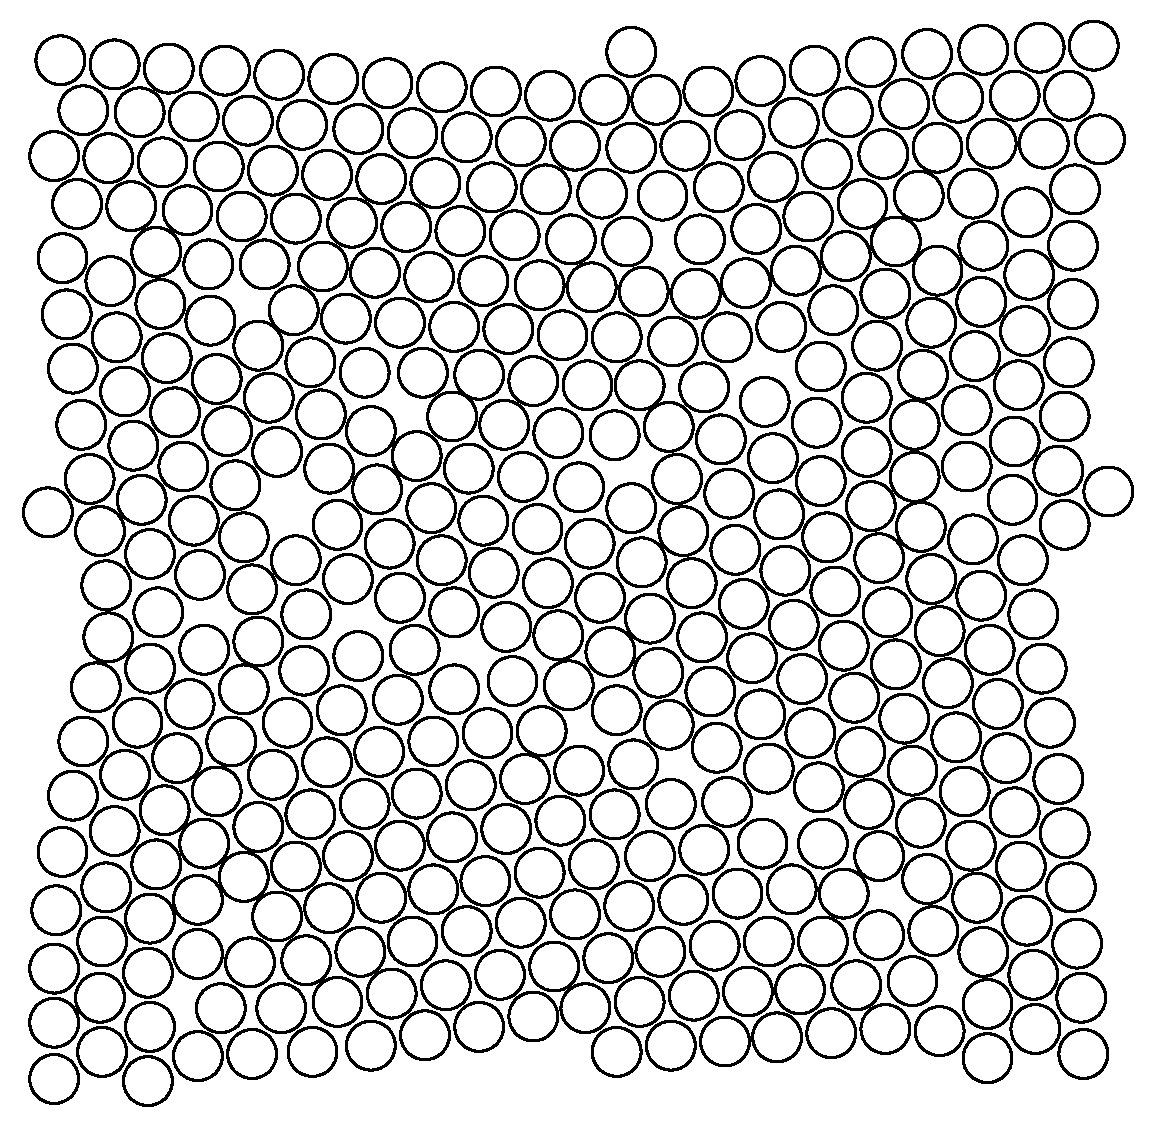
\includegraphics[width=\textwidth]{stepest.pdf}
			\caption{Steepest Descend}
		\end{minipage}
		\hspace{0.2\textwidth}
		\begin{minipage}[b]{0.25\textwidth}
			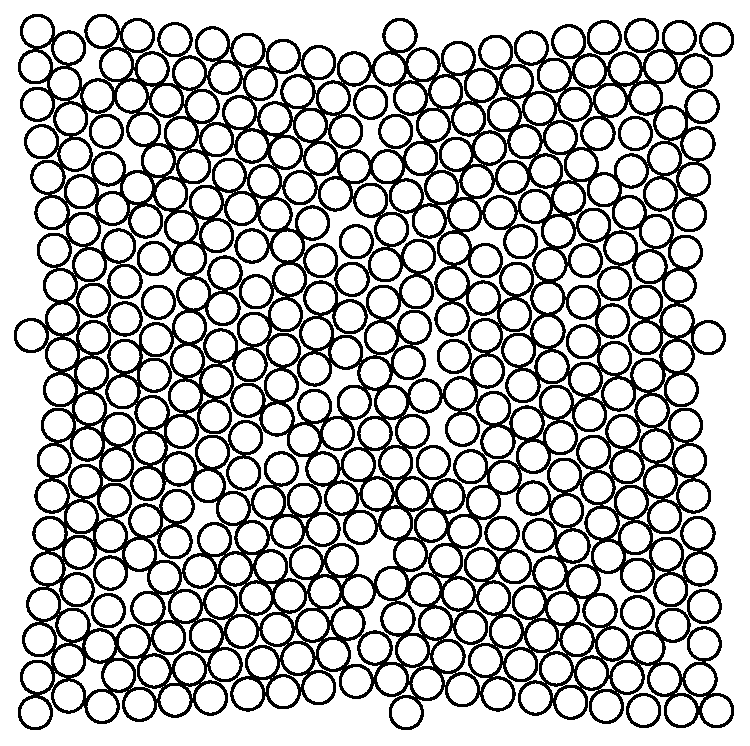
\includegraphics[width=\textwidth]{fire.pdf}
			\caption{Molecular Dynamics}
		\end{minipage}
		\caption{Compare two different methods}
	\end{figure}\\
	Look at the stucture, we found that they are extremely the same.
	\newpage
	\section{}
\end{document}